% !TEX encoding = UTF-8
% !TEX TS-program = pdflatex
% !TEX root = ../tesi.tex

%**************************************************************
\chapter{Progettazione}
\label{cap:progettazione}
Questo capitolo ha l'obiettivo di presentare l'architettura del prodotto e, se necessario, le motivazioni a favore delle scelte architetturali prese.
%**************************************************************

%**************************************************************
\section{Architettura}
    \subsection{Database}
    Viene presentata l'architettura del database relazionale mediante la \autoref{img:database}. Si noti che, in caso di relazione \textit{many-to-many}, la tabella \textit{pivot} non viene riportata in questo diagramma ma ne viene indicato il nome sulla relazione.

    \begin{figure}[p]
        \centering
        \hspace*{-2cm}
        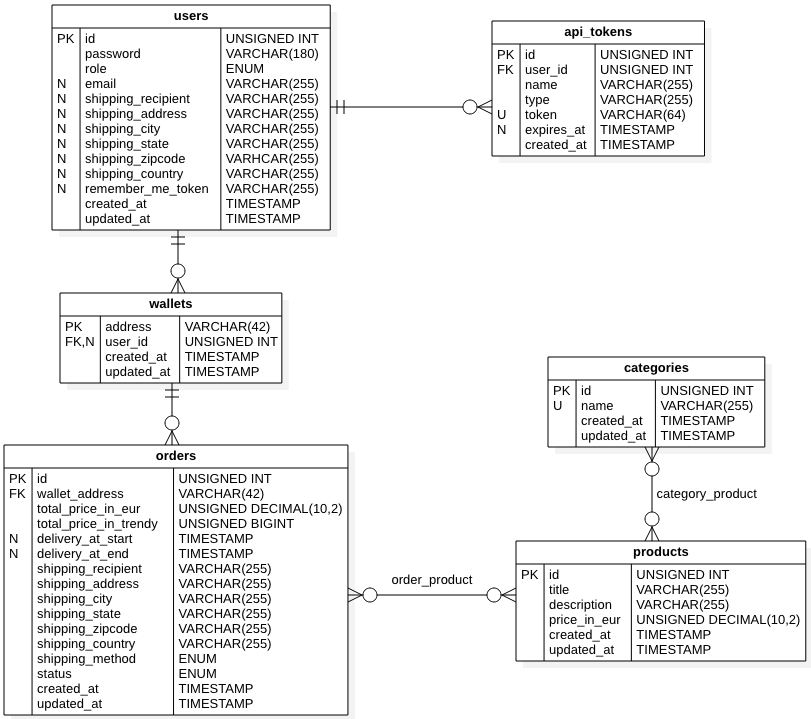
\includegraphics[width=16cm]{database.png}
        \caption{Diagramma Entità-Relazione del database}
        \label{img:database}
    \end{figure}

    \subsection{Back-end}
        \subsubsection{Idee generali}
        AdonisJS, in caso di utilizzo per la realizzazione di back-end che mettano a disposizione API REST, arriva out-of-the-box con una architettura monolitica basata sui principi della \textit{layered architecture} per i quali le dipendenze vanno da uno strato a quello immediatamente sottostante.
        \\\\
        In AdonisJS (così come in Laravel) è stato individuato un caso d'uso comune e sono stati forniti tutti gli strumenti per poterlo modellare efficacemente ed efficientemente. Questo caso d'uso è quello del back-end che accetta chiamate REST, sulla base di esse esegue delle operazioni di lettura scrittura su database e quindi prepara una risposta da ritornare al chiamante.
        \\\\
        Nella \autoref{img:architettura} notiamo tre diversi strati:
        \begin{enumerate}
            \item \textbf{API layer}: si occupa di definire: \textit{endpoint} REST, quali \textit{query param} sono accettati in ingresso ed eventuali middleware [\autoref{impl:middleware}] che il flusso di esecuzione dovrà attraversare prima di arrivare nei \textit{controller} ove verrà gestita la richiesta;
            \item \textbf{Business layer}: questo strato comprende i \textit{controller} che gestiscono la richiesta del front-end una volta attraversati i middleware; da qui può partire una richiesta di lettura/scrittura al database mediante il Persistence Layer e/o partire una richiesta a servizi esterni mediante appositi adapter;
            \item \textbf{Persistence layer}: si interpone fra Business Layer e Database facendo da traduttore mediante i modelli messi a disposizione dall'\textit{ORM} [\autoref{impl:orm}].
        \end{enumerate}

        \subsubsection{Adapter per servizi esterni}
        \label{proj:adapter}
        Al fine di aggiungere funzionalità non previste dal caso d'uso generale preso in considerazione da Adonis e mantenere il più possibile alta la manutenibilità dell'applicativo, si è fatto uso del pattern \textit{adapter} per disaccoppiare le classi controller dalle classi delle librerie web3.js [\autoref{img:adapter-web3js}] e CoinGecko-API [\autoref{img:adapter-coingecko}].

        \begin{figure}[h!]
            \centering
            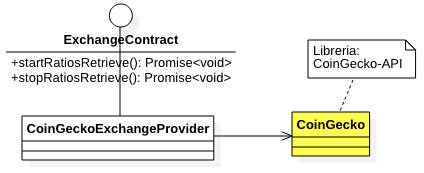
\includegraphics[width=9cm]{adapter-coingecko.png}
            \caption{Adapter per la libreria CoinGecko-API}
            \label{img:adapter-coingecko}
        \end{figure}

        \begin{figure}[h!]
            \centering
            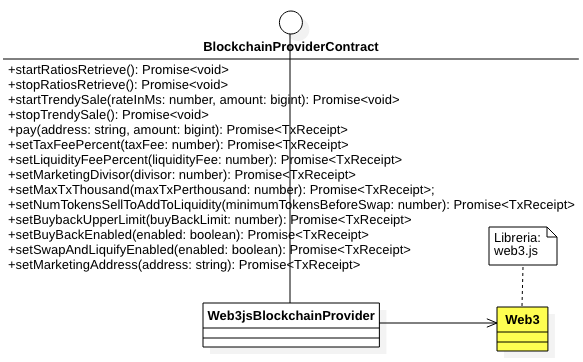
\includegraphics[width=14cm]{adapter-web3js.png}
            \caption{Adapter per la libreria web3.js}
            \label{img:adapter-web3js}
        \end{figure}


    \begin{landscape}
        \begin{figure}[p]
            \centering
            \hspace*{-4.5cm}
            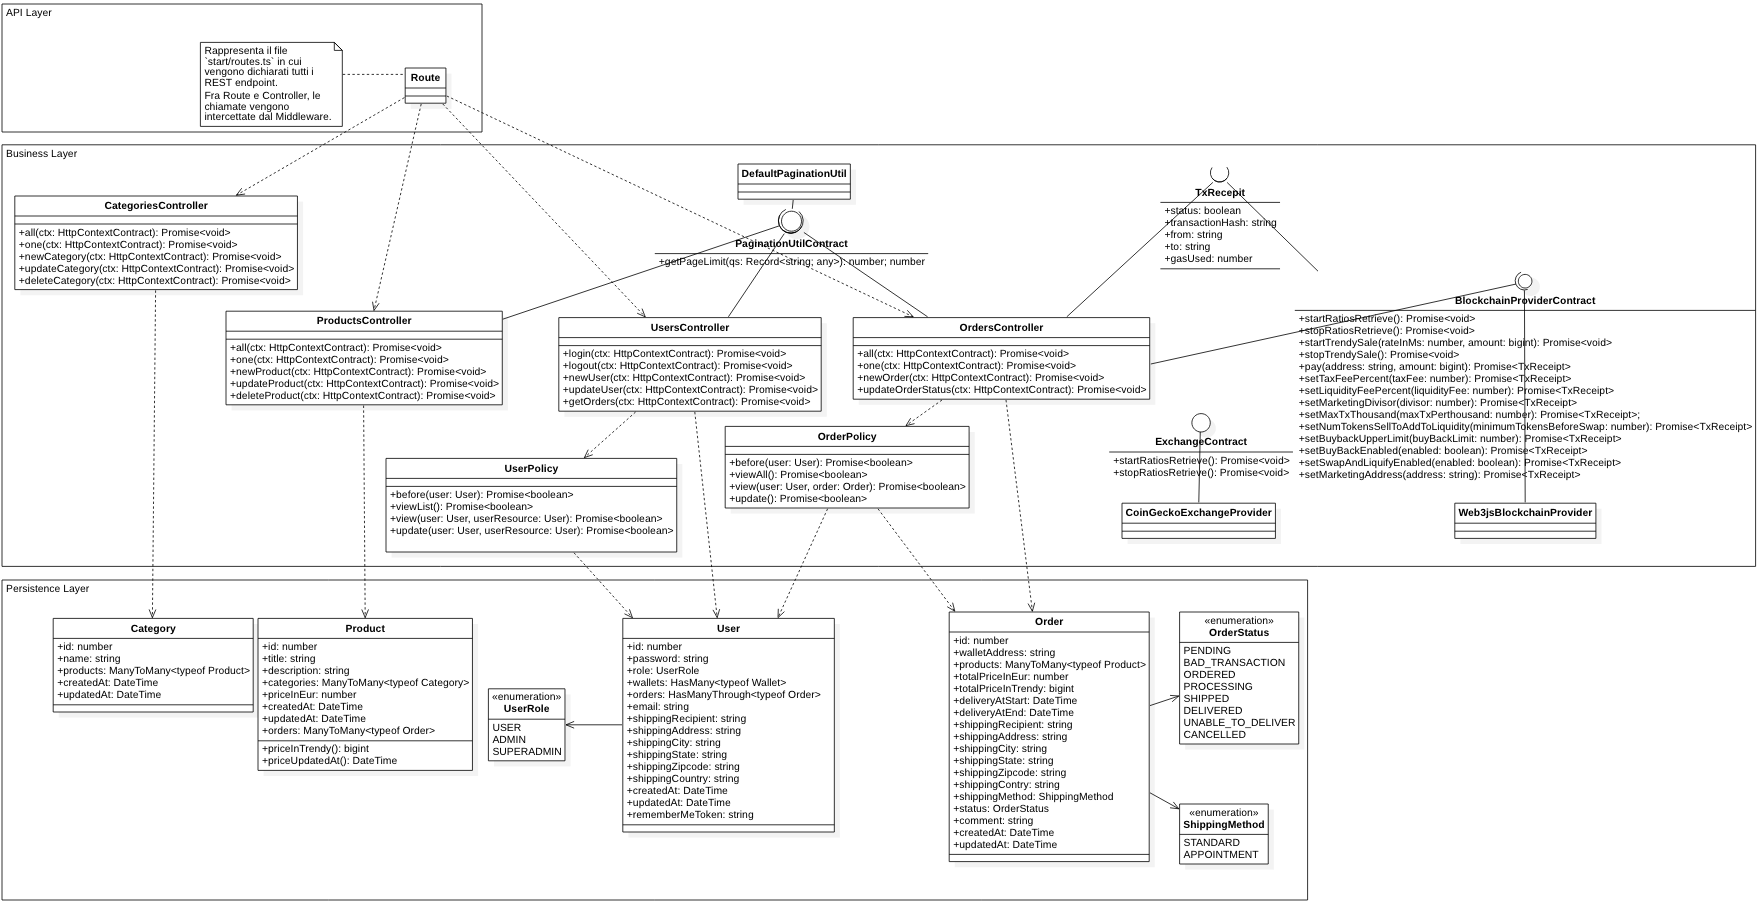
\includegraphics[width=28cm]{architettura.png}
            \caption{Diagramma UML delle classi del back-end con suddivisione in strati}
            \label{img:architettura}
        \end{figure}
    \end{landscape}